% Chapter 1

\chapter{Introduction} % Main chapter title

\label{Chapter1} % For referencing the chapter elsewhere, use \ref{Chapter1} 

\lhead{Chapter 1. \emph{Introduction}} % This is for the header on each page - perhaps a shortened title

%----------------------------------------------------------------------------------------
%\DeclareMathOperator*{\Min}{Min}
The problem addressed is to find a local minimizer of the nonsmooth minimization problem

\begin{equation} \label{mainproblem}
  \begin{aligned}
    & \underset{x \in \mathbb{R}^n}{\text{min}}
    & & f(x) \\
    & \text{s.t.}
    & & l_i \leq x_i \leq u_i , \; \\
    & & & i = 1, \ldots, n.
  \end{aligned}
\end{equation}

where $f \colon \mathbb{R}^n \to \mathbb{R}$, is continuous but not differentiable everywhere and $n$ is a very large but finite number.

The $L-BFGS-B$ algorithm \citep{lbfgsboriginal} is a standard method for solving large instances of \ref{mainproblem} when $f$ is a smooth function. The original name of $BFGS$ stands for Broyden, Fletcher, Goldfarb and Shanno, the authors
of the original "BFGS" quasi-Newton algorithm for unconstrained
optimization discovered and published
independently by them in 1970 \citep{Broyden} \citep{Fletcher} \citep{Goldfarb} \citep{Shanno}.
This method requires storing and updating a matrix which 
approximates the inverse of the Hessian matrix $\nabla^2 f(x)$ and
hence requires $\mathcal{O}(n^2)$ operations per iteration.  
The $L-BFGS$ variant \citep{MR572855} where the $L$ stands for ``Large'', is based on $BFGS$ but requires only $\mathcal{O}(mn)$ operations per iteration. And not only it requires less FLOPS, but it also requires much less memory. Instead of storing the $n \times n$ hessian approximations, $L-BFGS$ stores only $m$ vectors of dimension $n$, where $m$ is much smaller than $n$. Finally, the last letter B in 
$L-BFGS-B$ stands for bounds, meaning the lower and upper
bounds $l_i$ and $u_i$ in \ref{mainproblem}.  The $L-BFGS-B$ algorithm
is implemented in a well known \fortran software package
by the same name \citep{lbfgsbsoftware}

In this thesis, there is a brief description of the $L-BFGS-B$ algorithm
at a high level and then an explanation of how the modified algorithm
is more suitable for functions $f$ which may not be
differentiable at their local or global optimizers.  
We call the new algorithm L-BFGS-B-NS where NS stands for
Non-Smooth.  These changes were implemented in a modified version 
of the Fortran code \citep{lbfgsbNS} which can be downloaded from a web repository.  We report on some numerical experiments 
that strongly suggest that the new code should be useful for the
nonsmooth bound-constrained optimization problem (1.1).

We are grateful to Jorge Nocedal and his coauthors for allowing us 
to modify the L-BFGS-B code and post the modified version.  

%\chapter{deleted chapter}

%Larger problems not only mean that their solution will take a longer time to solve. But storing and calculating a the necessary matrices depends on the capabilities of the machine used to solve the problem and this might be prohibitively expensive. There a few large scale optimization techniques that have already been developed for the case when $n$ is very large. Also, several techniques have already been developed to handle this type of problems as long as the function $f$ is smooth. But there is not much out there about large scale problems with nonsmooth $f$

%In this thesis $f(x)$ is a nonsmooth function. This small change will require a few changes in the solution algorithm.

%For the particular case when $n$ is a small number, several methods that solve optimization problems of nondifferentiable functions in lower dimensions \citep{kiwiel85} have been developed. This thesis will try to see if it is possible to bring some of those concepts to large scale optimization. 

%In the case of smooth functions, it is possible to use Newton iteration algorithms and achieve quadratic convergence, the problem with Newton algorithms is that they require second derivatives to be provided\footnote{the main issue with the second derivative is that it requires a total of $n \times n$ partial derivatives. Which is impractical for medium and for some small-size problems}. In the 1950's and several years after that, several "quasi-newton" methods were proposed where the second derivative Hessian matrix is approximated step by step \citep{unconstrained}. These approximations or "updates" are calculated after every iteration of the original algorithm and the way in which this update is found defines a new method depending on the particular needs. This thesis will only be concerned with the $BFGS$. \footnote{BFGS stands for the last names of its authors Broyden, Fletcher, Goldfarb and Shanno} which can achieve super linear convergence, has proven to work in most practical purposes and posseses very nice self correcting features \citep{selfcorrecting}. In $BFGS$, it doesn't matter that one update incorrectly estimates the curvature in the objective function, $BFGS$ will always correct itself in just a few steps. This self-correcting property is very desired in the nonsmooth case, since changes in curvature could be abrupt near the optimal point. 

%$BFGS$ was originally developed for small to medium sized problems, and it is not the right tool for large scale optimization and therefore an $L-BFGS$ adaptation is needed to solve large scale problems\ref{mainproblem}. 

%A final assumption in this thesis is that the Hessian matrix is not sparse. In this case, there are other algorithms that may be more suitable \citep{Fletcher96computingsparse, sparse}, some of them have even been implemented in fortran \citep{lancelot}.

%This thesis builds upon the original $L-BFGS-B$ code \citep{lbfgsbsoftware} that solves smooth problems of $f$. There were three main changes in the code. The first one is the line search descent and curvature conditions which required a weaker version of the curvature in order to satisfy the different structure that a nonsmooth function requires. The second one is the line search methodology which was changed from a cubic interpolation to a bisection algorithm and last change in the thesis was the termination condition.

%Nocedal's original algorithm consists of $2$ steps. In the first step or gradient projection, most of the dimensions in the problem should be removed, making the problem a lot simpler. In the second step there is some fine tuning to guarantee better than just linear speed of convergence.

\chapter{L-BFGS-B}
\label{ChapterConstraints} % For referencing the chapter elsewhere, use \ref{ChapterConstraints} 

This section is a description of the original $L-BFGS-B$ code at a very high level \citep{lbfgsbsoftware}. The original software is intended to work well with smooth functions. This thesis discusses how to modify the algorithm for Non-Smooth functions. The original \textsc{FORTRAN} code contains as well some documentation \citep{codepaper} about how the software was built

\section{BFGS}

$BFGS$ is a standard tool for optimization of smooth functions.\citep{nocedal} It is a line search method and its goal is to find a search direction starting from its current position $x$. The search direction is of type $d = -B_k \nabla f$ \footnote{Notice that when $B$ is the identity, this is the same direction as steepest descent. Another common line search method of optimization} where $B_k$ is the $k^{th}$ approximation to the inverse Hessian. \footnote{When it is exactly the inverse Hessian the method is known as Newton's method. Newton's method has quadratic convergence but requires the explicit calculation of the Hessian at every single step.} This $k^{th}$ step approximation is calculated via the $BFGS$ formula

\begin{equation} \label{bfgsupdate}
  \begin{aligned}
    B_{k+1} = \left(I - \frac{s_ky_k^T}{y_k^Ts_k} \right) B_k \left( I - \frac{y_ks_k^T}{y_k^Ts_k} \right) + \frac{s_k s_k^T}{y_k^T s_k}
  \end{aligned}
\end{equation}

where $y_k = \nabla f(x_{k+1}) - \nabla f(x_k)$ and $s_k = x_{k+1} - x_k$ and where the first approximation of $B_0$ is assumed to be the the identity matrix $I$ in this thesis \footnote{a different starting matrix is suggested in Nocedal's book \citep{nocedal}}.  $BFGS$ exhibits superlinear convergence but it also requires $\mathcal{O}(n^2)$ operations per iteration. \citep{nocedal}

In the case of Non-Smooth functions. $BFGS$ typically succeeds in finding a local minimizer. This however requires some modifications of the line search conditions. This line search conditions are known as the Armijo and weak Wolfe line search conditions and they are a set of inequalities for computing an appropriate step length that reduces the objective function ``sufficiently''. These inequalities will be explained later in \ref{wolfeconditions}

\section{L-BFGS}

$L-BFGS$ stands for Limited-memory $BFGS$. This algorithm approximates $BFGS$ using only a limited amout of computer memory to approximate the inverse of the Hessian $B$. Instead of storing a dense $n \times n$ matrix, $L-BFGS$ keeps a record of the last $m$ iterations where $m$ is a small number that is chosen according to the problem at hand.\footnote{In this thesis $m < 20$, and in practice numbers between 5 and 10 are regularly used. There is no way of knowing a priori what choice of $m$ will provide the best results} It is for this reason that during the first $m$ iterations, $BFGS$ and $L-BFGS$ produce exactly the same search directions.

Because of this construction, the $L-BFGS$ algorithm is less computationally intensive and it only requires $\mathcal{O}(mn)$ operations per iteration. So it is much better suited for problems where the number of dimensions $n$ is large. For this reason it is the algorithm of choice in this thesis.

\section{L-BFGS-B}

Finally $L-BFGS-B$ comes naturally as an extension of $L-BFGS$. The $B$ stands for the inclusion of Boundaries.  $L-BFGS-B$ requires two extra steps on top of $L-BFGS$. First, there is a step called \emph{gradient projection} that reduces the dimensionality of the problem. Depending on the problem, the gradient projection could potentially save a lot of iterations by eliminating those variables that are at bound at the optimum thus reducing the initial dimensionality of the problem and the number of iterations and running time. After this \emph{gradient projection} comes the second step or \emph{subspace minimization}. During the \emph{subspace minimization} phase, an approximate quadratic model of \ref{mainproblem} is solved iteratively in a similar way that the original $L-BFGS$ algorithm is solved. The only difference is that during the search step phase the step length is restricted as much as necessary in order to remain within the box defined by \ref{mainproblem}.

\subsection{Gradient Projection}
The original algorithm was created for the case when $n$ is large and $f$ is smooth. Its first step is a gradient projection similar to the one outlined in \citep{gradproj1, gradproj2} which is used to determine an active set corresponding to those variables that are on either their lower or upper bounds. The active set defined at point $x^*$ is:

\begin{equation}
  \begin{aligned}
    \mathcal{A}(x^*) = \{ i \in \{1 \ldots n\} |  x^*_i = l_i \vee  x^*_i = u_i\}
  \end{aligned}
\end{equation}

Working with this active set is more efficient in large scale problems. A pure line search algorithm would have to choose a step length short enough to remain within the box defined by $u_i$ and $l_i$. So if at the optimum, a large number $\mathcal{B}$ of variables are either on the lower or the upper bound. At least a number $\mathcal{B}$ of iterations might be needed. Gradient projection tries to reduce this number of iterations. In the best case, only $1$ iteration is needed instead of $\mathcal{B}$.

Gradient projection works on the approximation model:

\begin{equation} \label{themodel}
  \begin{aligned}
    m_k(x) = f(x_k) + \nabla f(x_k)^T ( x - x_k) + \frac{(x - x_k)^T H_k (x - x_k) }{2}
  \end{aligned}
\end{equation}

where $H_k$ is a $L-BFGS-B$ approximation to the Hessian $\nabla^2 f$ stored in the implicit way defined by $L-BFGS$.

In this first stage of the algorithm a piecewise linear segment starts on the current point $x_k$ in the direction $-\nabla f(x_k)$. Whenever this direction encounters one of the constraints, the line segment turns corners in order to remain feasible. The path is nothing but the feasible piecewise projection of the negative gradient direction on the constraint box determined by the values $\overrightarrow{l}$ and $\overrightarrow{u}$. At the end of this stage, the value of $x$ that minimizes $m_k(x)$ restricted to this piecewise gradient projection path is known as the ``Cauchy point'' $x^c$.

\begin{figure}
\begin{center}
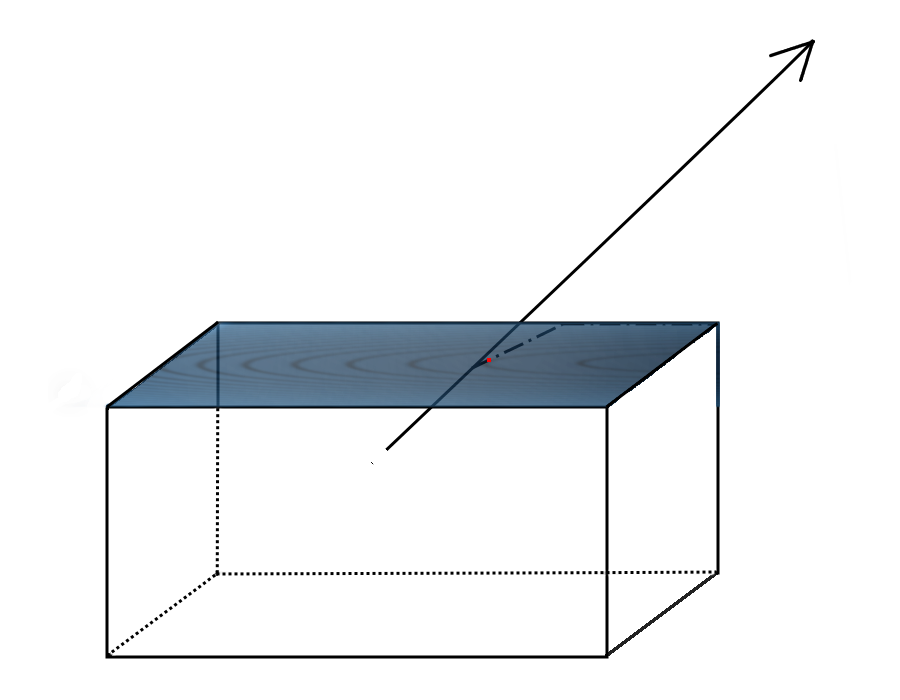
\includegraphics[scale=0.5]{Figures/cajapresentation2.png}
\caption[Graphical Representation of Gradient Projection]{The arrow represents the direction of the gradient. The dotted path represents the projected gradient path from the gradient and onto the box. The region represents the level sets of the model. The optimal point (in red) is the Cauchy point $x^c$}
\end{center}
\end{figure}

\subsection{Subspace Minimization}

The problem with gradient projection is that its search direction does not take advantage of information provided implicitly by the Hessian $H_k$, and therefore the speed of convergence is at best linear. It is for this reason that a stage two is necessary. Stage 2 or subspace minimization uses an $L-BFGS$ implicit approximation of the Inverse Hessian matrix restricted to the free variables that are not in the active set $\mathcal{A}(x^c)$.

The idea at a higher level is to solve the constrained problem \ref{themodel}, but only on those dimensions that are free. The starting point for this new stage will be the previously found Cauchy point $x^c$, the $L-BFGS$ algorithm provides a new search direction $\hat{d}^u$ that takes implicit advantage of second order approximations of the Hessian matrix.

The algorithm will move in the direction $\hat{d}^* = \alpha^* \hat{d}^u$ where $\alpha^*$ (the step length) is chosen so that the new point $\bar{x}_i$ satisfies Armijo and weak wolfe descent and curvature conditions, A third restriction on the step length is added so that the next iteration stays feasible. Once this step is finished, the next and final step will be the termination condition. If the termination condition fails, a new gradient projection and subspace minimization will be needed.

\chapter{Modifications to the L-BFGS-B algorithm}

We made three main changes to the original $L-BFGS-B$ algorithm. They concern the line search Wolfe conditions, the line search methodology, and the termination condition.

\section{The Armijo and Wolfe conditions} \label{wolfeconditions}

Probably the most important change made to the original code was the change in the curvature condition. It is accepted that the Armijo and Wolfe conditions work very well whenever the function $f$ is smooth \citep{MR1855221}. The Armijo condition, also known as the sufficient decrease requirement in the direction $d_k$ is defined as

\begin{equation} \label{armijocondition}
  \begin{aligned}
    f(x_k + \alpha_p d_k) \leq f(x_k) + c_1 \alpha_k d_k^T \nabla f(x_k)
  \end{aligned}
\end{equation}

where $0 < c_1 < 1$ is a constant usually $c_1 = 10^{-4}$\citep{nocedal}. This condition guarantees that the function continues decreasing and eventually reaches the optimum. It is possible to continue decreasing without ever reaching the optimum if the armijo condition is not required as is shown in figure~\ref{armijograph}

\begin{figure} 
\begin{center}
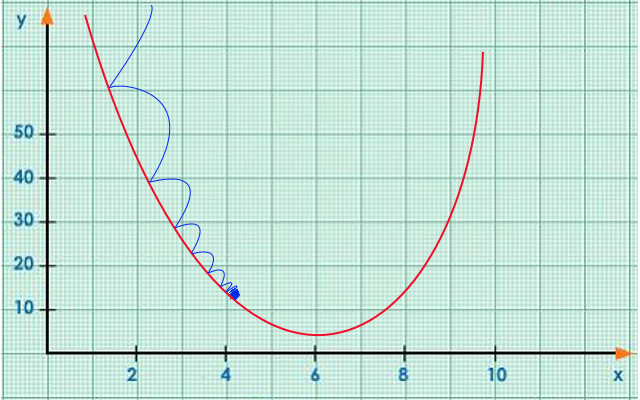
\includegraphics[scale=0.5]{Figures/armijo.png}
\caption[Representation of the Armijo Condition in a Nutshell]{In this figure, the iterations always reduce the value of the function a little bit, but never enough to go below $12$}
\label{armijograph}
\end{center}
\end{figure}

The other condition and the one that was actually changed, is the curvature condition, of which the most popular version is the ``strong Wolfe'' curvature condition:

\begin{equation} \label{strogwolfeq}
  \begin{aligned}
    |d_k^T \nabla f(x_k + \alpha _k d_k)| \leq c_2 |d_k^T \nabla f(x_k)|
  \end{aligned}
\end{equation}

Where $d_k$ represents the search direction and $c_2$ is a constant such that $0 < c_1 < c_2 < 1$ and is usually $c_2 = 0.9$\citep{nocedal}. The strong Wolfe condition is a natural choice for optimization of smooth functions. Its goal is to find a step length long enough that the slope has been reduced ``sufficiently'' as illustrated in figure~\ref{wolfefigure}, but the problem is that the condition as it is, does not work well for the Non-Smooth case. This is because near the minimal points there may be abrupt changes in the gradient. a good example of this problem is the function $f(x) = |x|$, where the slope never becomes flat near the optimal point.

\begin{figure} 
\begin{center}
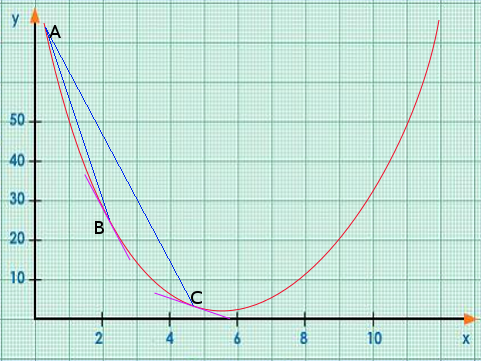
\includegraphics[scale=0.65]{Figures/wolfe.png}
\caption[The Idea behind the Wolfe Condition]{The logic of Wolfe conditions is this. Starting at point A. Point B is a step in the right direction, however, point C offers a ``flatter'' tangent and should be closer to the optimum which has a tangent of zero (Smooth case)}
\label{wolfefigure}
\end{center}
\end{figure}

The weak Wolfe condition defined as

\begin{equation}
  \begin{aligned}
    d_k^T \nabla f(x_k + \alpha _k d_k) \geq c_2 d_k^T \nabla f(x_k)
  \end{aligned}
\end{equation}

can be used in the Non-Smooth case. It is all that is needed to guarantee that the $BFGS$ updated inverse Hessian approximation is positive definite \citep{overtonlewis}. This weak version is suited for the problems in this thesis. It was changed inside of the line search algorithm explained in the next section.

\section{The line search methodology}

The original \textsc{FORTRAN} software\citep{lbfgsbsoftware} contains a line search subroutine. This subroutine originally consisted of three steps. This line search consists of finding a step length that satisfies a decrease and a curvature condition (the Armijo and Wolfe conditions from the previous section). This subprocedure was completely changed for the purpose of this thesis. The old version of the code was not removed, it was left commented out and is only explained here with the purpose of showing why it needed to be modified. It was called on line $2662$ \ref{ignoredcode} of \texttt{lbfgsbnomessages.f90} which is a file within the github repository\citep{lbfgsbNS}.

\begin{enumerate}
\item[First] the line search requires a maximum step. This maximum step is such that it guarantees that the step length stays within the bounding box delimited by $l$ and $u$, as such, this is a unique feature of the bounded algorithm$L-BFGS-B$. In the original \textsc{FORTRAN} code, this part of the line search was not changed.

\item[Second] an interval for $\alpha_k$ is chosen so that it contains a minimizer of the modified function,

\begin{equation} \label{armijomod}
  \begin{aligned}
    \Psi(\alpha_k) = f(x_k + \alpha_k d_k) - f(x_k) - c_1 \alpha_k d_k^T  \nabla f(x_k)
  \end{aligned}
\end{equation} 

 which is nothing but a modification of the Armijo condition\ref{armijocondition}. If $\Psi(\alpha_k) < 0$ and $\alpha_k d_k^T \nabla f(x_k) > 0$. The interval contains a minimizer of $f$ and the subroutine can continue to the next step. This first stage took place in the subroutine $dcsrch$; specifically on lines $3687$ and $3709$\ref{stage2}.

\item[Third] stage is the typical line search\citep{nocedal}. It was called on line $3713$ of \texttt{lbfgsbnomessages.f90} and its mission was to find the step that satisfied Armijo and ``Strong'' Wolfe conditions on the original function $f$. Both steps 2 and step 3 are called on the subroutine $dcstep$. The subroutine still exists on file \texttt{lbfgsbnomessages.f90} for illustration. Although it is only commented out and never called in this thesis.

\end{enumerate}

Those three steps make up the original subroutine. But there is a problem with the function $dcstep$ on the third step as it concerns this thesis. It turns out that function $dcstep$ was designed to work only with smooth functions in mind. The algorithm takes advantage of quadratic and cubic approximations to the function in order to calculate the next points that satisfy Armijo and Wolfe conditions. Unfortunately, these second and third order approximations do not work in the Non-Smooth case, and the optimizer crashes under the line search as it is. Function $dcstep$ starts on line $3779$ and a sample of the approximations is shown in between lines $3881$ and $3902$ \ref{nsnowork} of \texttt{lbfgsbnomessages.f90}.

The solution to this particular issue is to use a line search similar to the one implemented in hanso \citep{hanso}. The HANSO approach is to double the step length while the Armijo condition is violated. And once the interval has been bracketed, to do a bisection until both Armijo and Wolfe conditions are satisfied. The only difference with the HANSO approach in this thesis is that the line search in HANSO can double its step length up to $30$ times \footnote{for all practical purposes this is considered a good limit of iterations}. Whereas in this thesis, the step length can double only as long as the step length is less than the maximum value that guarantees feasibility of the solution (the maximum stablished in the first step of the original line search). This version of the bisection and expansion is found in between lines $4425$ and $4456$ of \texttt{lbfgsbnomessages.f90}\ref{linesearchww} 

\section{The Termination Condition} \label{terminator}

One important requirement of an algorithm is that it ends in a finite time. In the case of smooth functions, $L-BFGS-B$ checks whether the algorithm has converged, by means of the \emph{projected gradient} which is nothing but the projection of the negative gradient onto the bounding box defined by $l$ and $u$. If this projected gradient has a small norm\footnote{smaller than some tiny $\epsilon > 0$} the algorithm has converged. In the case of Non-Smooth functions however, this is not necessarily true and the function at the minimum may have a wedge. In this wedge the projected gradient may not vanish. Furthermore, if there is a sequence of points that approaches the optimum $x$ in a direction \vec{p}, the projected gradients corresponding to this sequence of points might be completely different from the projected gradients associated to a sequence of points that approach the optimum $x$ from an opposite direction.

Given this set of conditions, there is a need for particular rules to establish the finalization of the optimization, these rules have already been established in some works before\citep{overtonlewis} \citep{skajaa}.

\subsection{Description of the Solution}
%Warning review
Overton and Lewis formulate an algorithm that gives a practical solution to this problem on section $6.3$ \citep{overtonlewis}
The best practical methodology should be to calculate wheter zero $0$ or a very small number is the norm of a vector that is part of the convex hull of gradients evaluated at points near the optimum candidate $x$. The neighborhood is defined as those points with a distance to $x$ smaller than a small tolerance $\tau_x > 0$ and no more than $J \in \mathbb{N}$ iterations back. In order to make sure that the gradient zero $\vec{0}$ or a vector with a very small norm smaller than a very tiny tolerance $\tau_d > 0$ is part of the convex hull calculated near a neighbourhood of the optimum, the algorithm  keeps a record of the latest gradient vectors in this small neighbourhood of the point where the optimum is suspected to be located. This list of gradients is referred to as the set $\mathcal{G}$ \citep{overtonlewis}

With this list $\mathcal{G}$ of gradients at hand. The next step is to find the vector with the minimal norm contained in the convex hull of these gradients.  If the norm of this vector has a norm smaller than $\tau_d$ , the algorithm ends with a message of convergence success. If the minimum such norm is larger than the tolerance, the algorithm must continue to the following iteration and not terminate.

In order to find this vector, there is the need to solve a quadratic problem. Every vector in the convex hull can be expressed as a nonnegative linear combination $Gz$ of those vectors in $\mathcal{G}$. Where $G$ is the matrix with columns made up of gradients in $\mathcal{G}$; and $z$ is such that $\sum_{i=1}^n z_i = 1$ and $z_i \geq 0$.

The objective is to find the right combination of $z$ that minimizes the norm $||Gz||_2$.  This is equivalent to solving the following optimization problem

\begin{equation} \label{quadraticproblem}
  \begin{aligned}
    & {\text{min}}
    & & q(z) = ||G z ||_2^2 = z^TG^TGz  \\
    & \text{s.t.}
    & & \sum_{i = 1} ^J z_i = 1 \; \\
    & & & z_i \geq 0.
  \end{aligned}
\end{equation}

The solution to this problem $z^*$ has the associated vector $Gz^*$. And if $||Gz^*||_2 < \tau_d$ the algorithm converges.

\subsection{The Solution of the Quadratic Program}

The solution of \ref{quadraticproblem} was implemented with a practical primal-dual methodology. This methodology is the same methodology implemented by Skajaa \citep{skajaa} in his thesis. His code \textsf{qpspecial} was implemented in \textsc{FORTRAN} for this thesis and is part of \texttt{lbfgsbnomessages.f90}. His algorithm solution is the well known Mehrotra's Predictor-Corrector algorithm implementation applied to quadratic programming.

This algorithm initially tries to solve the Karush-Kuhn-Tucker $KKT$ conditions. The $KKT$ is a system of equations whose solution characterizes the solution of the original optimization problem. In \ref{quadraticproblem}, the Karush Kuhn Tucker equations are:

\begin{equation} \label{kkt}
  \begin{aligned}
    G^TGz - e^Ts
    & = & 0 & \\
    \sum_{i = 1}^J x - 1
    & = & 0 & \\
    z_is_i & = & 0 &; &i = 1,2, \dots, J\\
    (s, z) & \geq & 0 &
  \end{aligned}
\end{equation}

Where $s$ is the variable that represents the dual problem.

In order to solve this system of equations a variant of Newton's method is used. The method provides a search direction and as usual for this type of methods, it  requires a corresponding step length. Since this is an interior point method, it approaches the solution following a path inside the convex interior of the feasible set.  In the best of cases, it would be nice to approach the solution through a \emph{central path} defined as third equation in \ref{kkt} is allowed to take more relaxed values $z_is_i = \tau$, where $\tau \geq 0$. If the solution is approached through this \emph{central path}. The convergence will require fewer iterations \footnote{The reason why the central path is so convenient is more thoroughly explained in Nocedal's text chapter $14$\citep{nocedal}}.

The problem with a pure Newton's method is that it's solution is not close to this \emph{central path}. The step length is usually very small because of the nature of the third and fourth equations. For this reason, if the step length is too large, the condition of $z > 0$ or $s > 0$ will be violated and unfortunately, the pure method as it is does not allow reasonable step sizes in practice. The method approaches the solution very close to the boundaries of the feasible set and far away from the \emph{central path} where the step lengths could be larger and the convergence therefore would be faster. It is for this reason that a \emph{centering} of the path is performed. This first step is known as the ``predictor'' step.

Besides the centering; Mehrotra proposed a ``correction'' stage which pushes the solution even closer to the \emph{central path} by taking into account its curvature. This second stage is also used to calibrate some of the parameters used during the centering in the ``predictor'' stage\footnote{These are some parameters that calibrate the speed at which the tangent path is pushed into the central path. This is also explained in chapter $14$\citep{nocedal}}. The second stage is similar to the first stage in that it requires the solution of a new system of equations.

\begin{figure}
\begin{center}
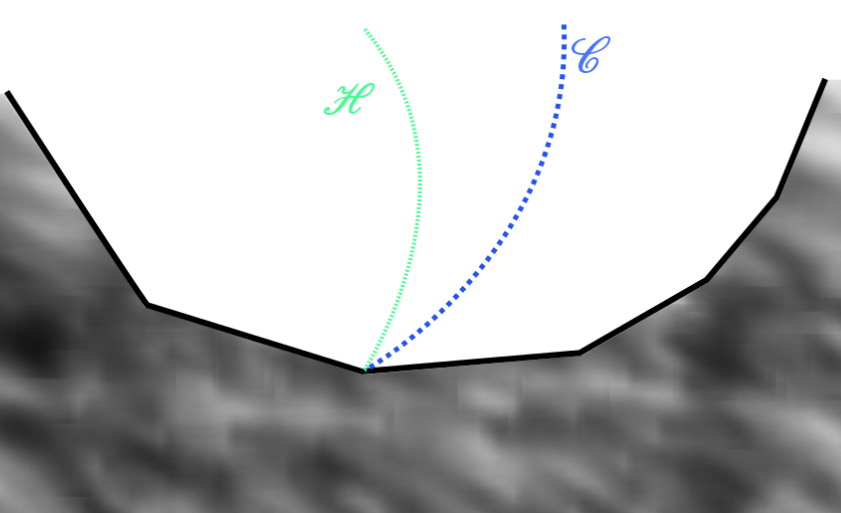
\includegraphics[scale=0.3]{Figures/CentralPath.png}
\caption[The Central Path and the Tangent Path]{The central path $\mathcal{C}$ is approached from a current and noncentral point on the tangent path $\mathcal{H}$}
\end{center}
\end{figure}

And this is very important, because both steps require a solution of a system of equations which in turn requires a matrix factorization. And this factorization can be recycled. Mehrotra's algorithm requires only one Cholesky factorization for the first stage. This factorization is reused during the second stage. By reusing the factorization, the performance is improved.

\chapter{Solution Tests}

The $L-BFGS-B$ implementation was tested on the high performance cluster machines at NYU. In order to run these tests it was necessary to create a series of PBS files using a PBS generator script \ref{pbsgenerator}. This script generator created PBS files which in turn run bash scripts \ref{pbsfile}. The main reason to run scripts this way is because it achieves parallelism, and because the system sends confirmation e-mails and statistics about the different stages of the processes giving a lot of control to the practitioner. The original $L-BFGS-B$ optimizer displays different messages depending on the initial condition that triggered the exit.  

\section{Exit Messages}

The following is a list of some of the other most common exit messages in the original $L-BFGS-B$ optimizer.

\begin{itemize}

\item 'ABNORMAL\_TERMINATION\_IN\_LNSRCH' This message means that there was a problem and a premature exit was required. It is typically found in Non-Smooth functions where the cubic interpolation is impossible. But the message is also symptomatic of other problems.

\item 'CONVERGENCE: NORM\_OF\_PROJECTED\_GRADIENT\_LT\_PGTOL': Means that convergence was achieved because the norm of the projected gradient is small enough. Notice that this convergence message does not apply to $L-BFGS-B-NS$ because of particular requirements for Non-Smooth functions involving the convex hull instead\ref{terminator}.
\item 'CONVERGENCE: REL\_REDUCTION\_OF\_F\_LT\_FACTR*EPSMCH': This convergence condition is achieved whenever the relative reduction of the value of function $f$ is smaller than a predefined factor times machine $\epsilon$.

\item 'ERROR: N .LE. 0': This is one of many error checks performed at the beginning of the execution.

\item 'ERROR: NO FEASIBLE SOLUTION': An error condition for those cases when the solution is not feasible. This is because the original $L-BFGS-B$ optimizer allows oppen boxes of type [$l$, $\infty$[, ]$-\infty$, $u$] and ]$-\infty$, $\infty$[

\item 'WARNING: ROUNDING ERRORS PREVENT PROGRESS': If there is a rounding error issue

\end{itemize}

on top of these messages, $L-BFGS-B-NS$ introduced a new message for a succesful exit from its termination condition\ref{terminator}

\begin{itemize}
\item 'CONVERGENCE: ZERO\_GRAD\_IN\_CONV\_HULL' What this means is that all termination conditions\ref{terminator} were satisfied\footnote{This does not mean that the resulting vector is exactly equal to zero $0$, but it is small enough to finish the execution of the algorithm}.
\end{itemize}

\section{Modified Rosenbrock Function} \label{ros}

With those tools in hand, it is possible to run a few tests of the algorithm. Several functions were evaluated. One of them is a modified version of the Rosenbrock function problem\citep{rosenbrock}:

\begin{equation} \label{modifiedrosenbrock}
    f(x) = (x_1 - 1)^2 + \sum_{i = 2}^n |x_i - x_{i - 1}^2|^p
\end{equation}

Here, the properties of the function depend on the value of $p$\footnote{The original Rosenbrock function would have a value of $p = 2$}. This function can be proven to be locally lipschitz continuous whenever $p \geq 1$. In particular it is Locally Lipschitz continuous if restricted to a finite domain of the type $l$, $u$, similar to the one defined on\ref{mainproblem}.

The region to be tested is defined by the ``box'' with boundaries

\begin{equation}
  \begin{aligned}
    x_i = 
    \begin{cases}
      [-100, 100] & \text{if } i \in \text{ even numbers} \\
      [10, 100] & \text{if } i \in \text{ odd numbers}
    \end{cases}
  \end{aligned}
\end{equation}

And the initial point was chosen to be the midpoint of the box, plus a small perturbation chosen so that the search direction does not reach the boundary of several dimensions in one stroke.

\begin{equation}
  \begin{aligned}
    x_i = \frac{u_i - l_i}{2} - (1 - 2^{1 - i})
  \end{aligned}
\end{equation}

The problem is smooth for values of $p$ close to $2$, but as the values of $p$ approach $1$, the original $L-BFGS-B$ optimizer should start to have problems. In order to check for that, we plug the Modified Rosenbrock function into the original $L-BFGS-B$ optimizer with $p$ parameters varying between $2$ and $1$. 


\begin{figure}
\begin{center}
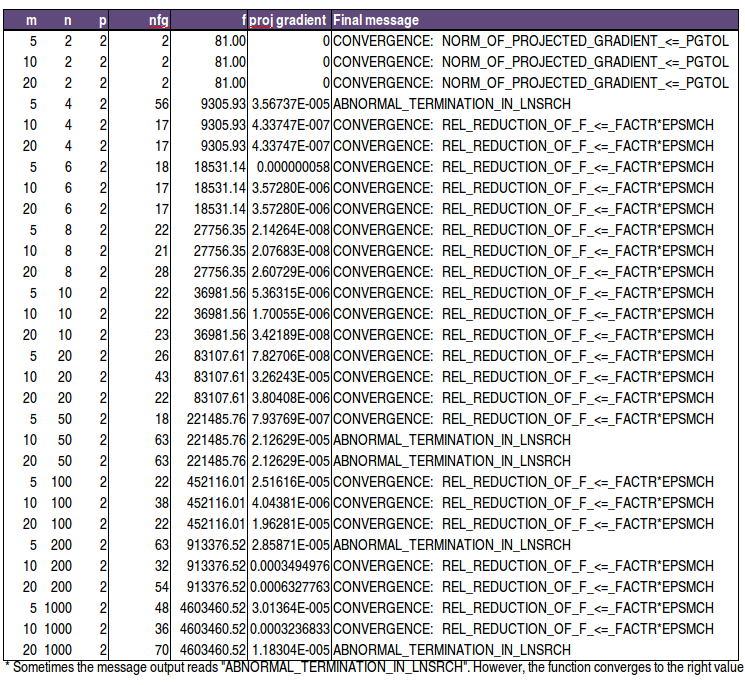
\includegraphics[scale=0.58]{Figures/Nocedalp2.png}
\caption[Modified Rosenbrock with $p = 2$]{Satisfactory results for the original algorithm $L-BFGS-B$ applied to the Modified Rosenbrock function with $p = 2$}
\label{pequal2}
\end{center}
\end{figure}


For a value of $p = 2$, the original $L-BFGS-B$ optimizer does not have too many problems and it yields good results as seen on the resulting table\ref{pequal2}.

This exercise tested three different values of $m$, where $m$ stands for the steps in memory of $L-BFGS$. The steps that were tested are $5$, $10$ and $20$, because they cover more or less the set of recommended values. The number of dimensions in this exercise in particular ranges from $2$ to $1000$ and covering many values in between. The column $nfg$ stands for the number of iterations taken in order to finish the algorithm and $f$ stands for the optimal value that was achieved during the optimization. The two last columns stand for the norm of the projected gradient and the final message when the algorithm finished.

In all cases the projected gradient has a very small norm. When this norm is tiniest the convergence is achieved because the norm of the projected gradient is smaller than the threshold. In other cases, the program exits succesfully after a relative reduction in the size of the function. In other cases, an abnormal termination message is sent to the output.

Notice that in \ref{pequal2} the program sometimes sends a warning message even though the function has converged to a value that more or less is very close to the optimal expected value.  This is because the original Rosenbrock function is designed to be very difficult to solve.  Its minimum is located in a banana shaped valley. This valley is very flat and is supposed to cause trouble to even the best optimizers as seen in figure \ref{dualgraph}

\begin{figure}
\centering
\mbox{\subfigure{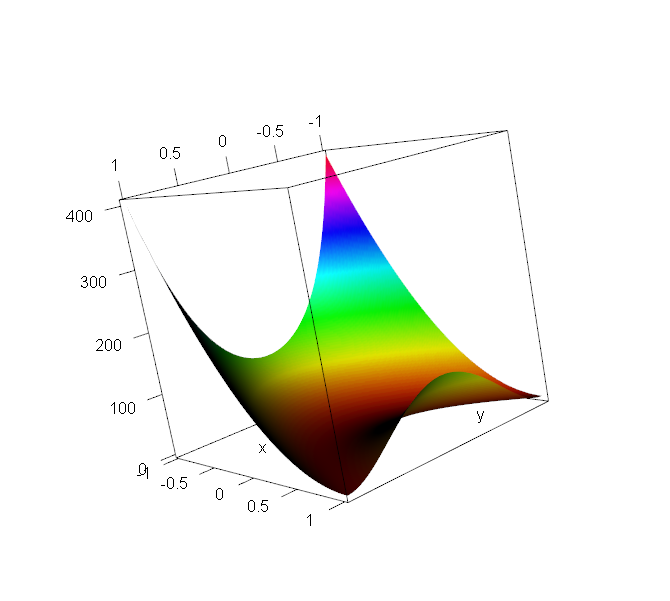
\includegraphics[scale = 0.4]{Figures/rosenbrock.PNG}} \quad
\subfigure{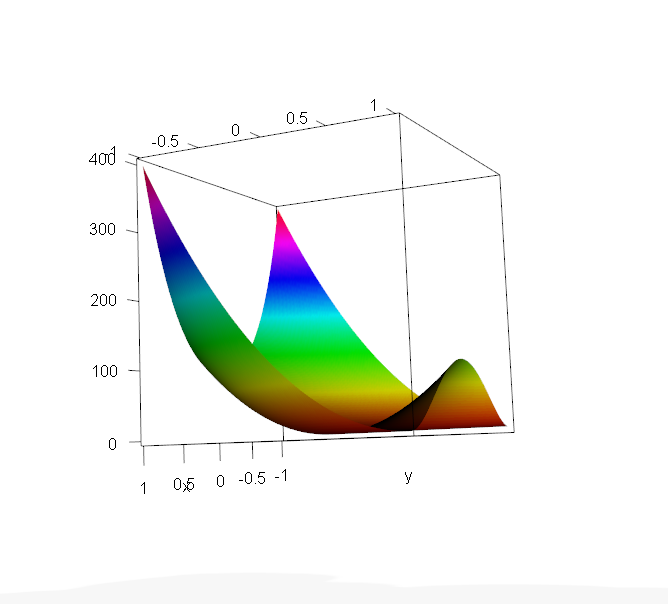
\includegraphics[scale = 0.4]{Figures/FlatBottom.PNG} }}
\caption[Original Rosenbrock Function Mesh]{The original Rosenbrock function $f(x,y) = (1 - x)^2 + 100(y - x^2)^2$ is designed to be a very difficult function to optimize. The global minimum is located along the very narrow, flat banana shaped valley\citep{rosenbrock}}
\label{dualgraph}
\end{figure}

It is perhaps easier to see it all on the contour plot \ref{contourbanana}

\begin{figure}
\begin{center}
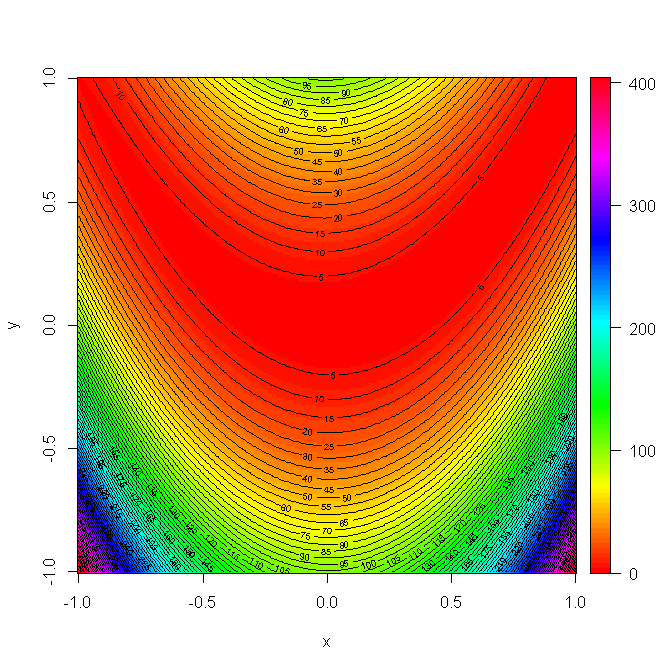
\includegraphics[scale=0.5]{Figures/contour.PNG}
\caption[Contour Plot of the Original Rosenbrock Function]{The contour plot shows the valley in red where the global optimum is located}
\label{contourbanana}
\end{center}
\end{figure}

The overall conclusion from this exercise is that the original $L-BFGS-B$ optimizer works well, for the smooth Rosenbrock case\footnote{The original algorithm solves a modified version of this function \ref{modifiedrosenbrock}, so it is to be expected that the performance is good}.

\begin{figure}
\begin{center}
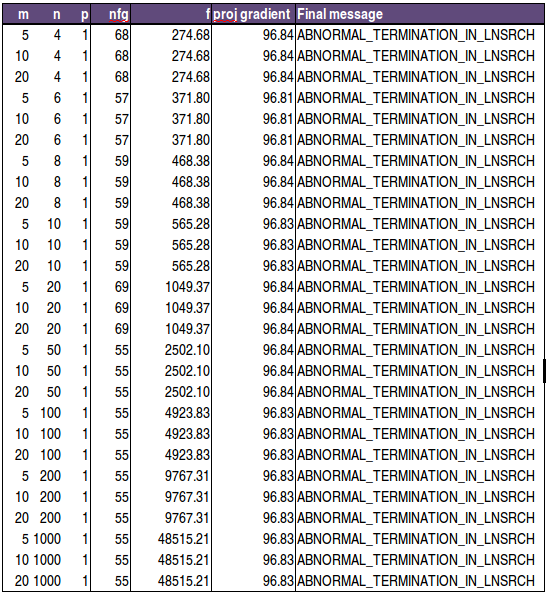
\includegraphics[scale=0.5]{Figures/abnormalNocedal.png}
\caption[Modified Rosenbrock with $p = 1$]{Unsatisfactory results for the original algorithm $L-BFGS-B$ applied to the Modified Rosenbrock function with $p = 1$, notice however that the two-dimensional case is succesful.  This is because the function is smooth in this particular case.}
\label{pequal1}
\end{center}
\end{figure}

On the other hand, the value of $p = 1$ has an abnormal line search termination in all of the cases presented. The projected gradient values are always far away from zero. The memory length $m$ of $L-BFGS$, does not have an impact in the final value $f$ of the optimization, but this is because all cases crashed before the $5^{th}$ iteration and therefore all different cases of $m$ end up looking exactly the same in this table.

By the same token several other values of $p$ were also tested, among others $1.5$, $1.1$, $1.01$, $1.001$, ... , $1.000000001$, $1$. As expected, those values where $p$ is closer to $1$ give the most problems to the original algorithm. When $p=1$ the algorithm does not work as seen in \ref{pequal1}\footnote{This is expected because the algorithm is originally designed to handle only smooth functions}.

For intermediate values, the new changes seem to provide better values of $f$. Here is a simple comparison of the algorithm running on $m = 5,10$ for selected values of $p$ \ref{pcomp}

\begin{figure}
\begin{center}
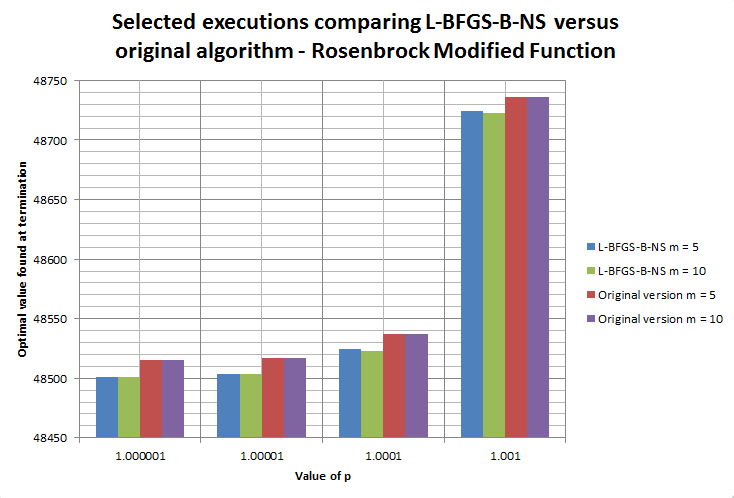
\includegraphics[scale=0.75]{Figures/ComparisonNewOld.PNG}
\caption[Comparison of selected values of the Modified Rosenbrock function]{Comparison of the performance of $L-BFGS-B-NS$ vs. the Original version of $L-BFGS-B$ applied to the Modified Rosenbrock function with selected values of p in 1.000 dimensions}
\label{pcomp}
\end{center}
\end{figure}

These are typical values of optimizations for intermediate values of $p$. In the bar graph it is possible to see that values generated via $L-BFGS-B-NS$ are a little better for values of $p$ closer to $1$. Finally, there is a table with the number of evaluations performed sliced by $p$ and $m$ \ref{pmtable}. And just as it would be expected, the number of evaluations required is higher for values of $p$ close to $1$.

\begin{figure}
\begin{center}
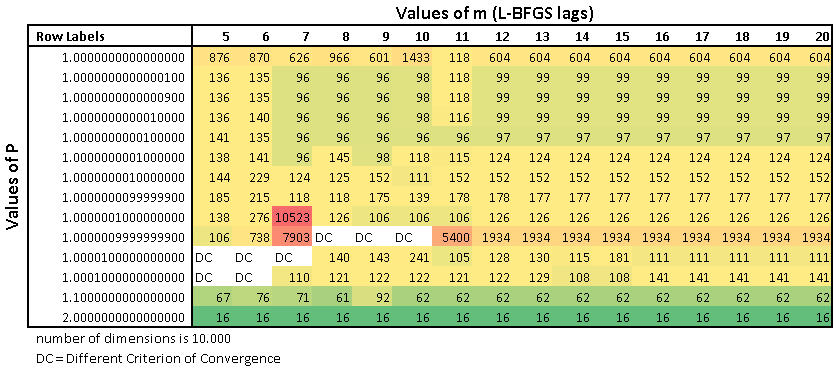
\includegraphics[scale=0.75]{Figures/Niterations.PNG}
\caption[Number of function evaluations for different values of $p$ and $m$ in the solution of Modified Rosenbrock]{This is the number of function evaluations for different values of $p$ and $m$. The number of function evaluations is a few times higher than the number of iterations because it iterations requires to evaluate the function a couple of times for the line search. Values of DC converged using other stopping criteria besides the termination condition \ref{terminator}}
\label{pmtable}
\end{center}
\end{figure}

\section{Nesterov's Chebyshev-Rosenbrock Modified function}

This function is a Non-Smooth variation of \texttt{NCR-NS1} which was first introduced in the thesis by Kaku\citep{kaku}. The function is defined very similar to \ref{modifiedrosenbrock}.

\begin{equation} \label{modifiedyurirosen}
    f(x) = \frac{(x_1 - 1)^2}{4} + \sum_{i = 1}^{n-1} |x_{i+1} - 2x_{i}^2 + 1|^p
\end{equation}

Where the $p$ is also assigned as a control variable for the Lipschitz Continuity of the function. The problem as stated in Kaku's thesis, is that the manifold defined by the term inside the sum, also known as:

\begin{equation} \label{kakumanifold}
    M = \{x: x_{i+1} - 2x_i^2 + 1 = 0, i = 1, \hdots, n-1 \}
\end{equation}

is highly oscillatory in nature, and therefore $BFGS$ methods require many iterations to converge. In particular, the next table tries to slice the number of iterations required to finish the algorithm given different combinations of $p$ and $n$, the number of dimensions\ref{yuripn}.

\begin{figure}
\begin{center}
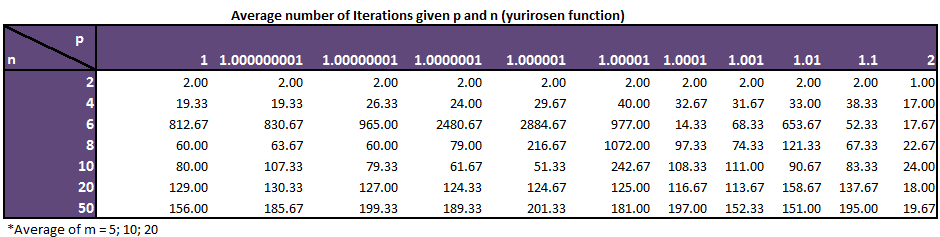
\includegraphics[scale=0.6]{Figures/yurirosenpn.PNG}
\caption[Comparison of selected values of the Modified NCR-NS1 function sliced by p and n]{Comparison of the number of iterations in order to converge for the Modified NCR-NS1 functions sliced by the number of dimensions $n$ and the $p$ parameter that controls the Smoothness of the function}
\label{yuripn}
\end{center}
\end{figure} 

The results show that the number of iterations increases significatively with smaller values of $p$, and in general with larger values of the dimension $n$. The number of iterations is a lot larger than for the previous case \ref{ros} 

This table was also sliced with the parameters $n$ and $m$ in figure \ref{yurimn}.

\begin{figure}
\begin{center}
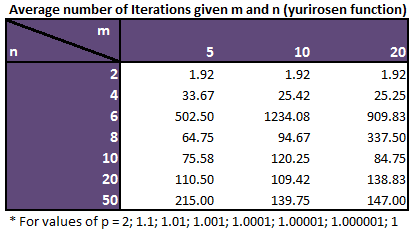
\includegraphics[scale=0.9]{Figures/yurirosenmn.PNG}
\caption[Comparison of selected values of the Modified NCR-NS1 function sliced by m and n]{Comparison of the number of iterations in order to converge for the Modified NCR-NS1 functions sliced by the number of dimensions $n$ and the memory lag $m$}
\label{yurimn}
\end{center}
\end{figure} 

\chapter{Conclusions}

%-------------------------------------------------------------------------
The need to build optimizers that work on a large number of variables quickly led us to the use of large scale quasi-Newton methodologies. These methodologies have been show to work very well for smooth functions and several implementations have been suggested in the literature and some implementations are already available.

Implementing the changes proposed to the original $L-BFGS-B$ software like changing the Wolfe condition from the strong to the weak version and using a line search algorithm that does not require smoothness of the function at critical points, provides the capability to run optimizations on Non-Smooth functions on simply restricted domains.

With the new tool, which is called $L-BFGS-B-NS$, it is possible to run optimizations of problems that involve a few millions of variables for some complicated test functions. The software has been tested with very challenging functions and has performed well.

The new methodology offered some challenges to the way in which the algorithm terminates and for this reason it was also necessary to implement termination conditions that take care of the wedges natural to Non-Smooth functions. The new termination conditions work fine for the problems tested.

After running the algorithm it seems like there is not a good rule to choose the number of memory step terms $m$ to keep in memory, but this is something that also happened in the case of smooth functions. Also, the test functions Modified Rosenbrock and Modified NCR-NS1, show that the most complicated and quasi-Non-Smooth a function becomes, the more iterations and function evaluations will be required for the function to converge.

Another conclusion, quite obvious, is that larger problems involve a greater number of ressources

Future steps suggest the investigation of limited-memory bundled methods $LMBM$, how it compares with $L-BFGS-B-NS$ and how one could benefit from the other. Also, the study of the impact of the Lipschitz constant on the convergence of the $L-BFGS-B-NS$ algorithm\citep{QJ:QJ935}.

